\section{Приклад застосування для не супермодулярної задачі}
Наразі невідомо, яким є співвідношення між кількістю супермодулярних задач та кількістю тих задач, 
які може розв'язувати наведений алгоритм. Водночас цей приклад свідчить про те, що
що множина не супермодулярних задач, які наведений
алгоритм може розв’язувати, не є пустою.


Використаємо представлений алгоритм для невеликої $(\max,+)$ задачі розмітки для ілюстрації.
Візьмемо довільне додатне парне число $x\geq 10$. Нехай задачу задано множиною
об'єктів $T=\{t_1,t_2,t_3,t_4\}$, структурою сусідства \\$\Gamma=\{(t_1,t_2),(t_1,t_3),(t_2,t_4),(t_3,t_4)\}$, 
множиною міток $K=\{0,1,2\}$, якостями вершин 
\begin{equation*}
    \begin{aligned}
       q_{t_1}(0)=q_{t_2}(0)=q_{t_3}(0)=0,\\
       q_{t_1}(1)=q_{t_2}(1)=q_{t_3}(1)=-\frac{x}{2},\\
       q_{t_1}(2)=q_{t_2}(2)=q_{t_3}(2)=-x,\\
       q_{t_4}(0)=-x+1,\\
       q_{t_4}(1)=-\frac{x}{2}-1,\\
       q_{t_4}(2)=-1,
    \end{aligned}
\end{equation*}
і якостями ребер 
\begin{equation*}
    g_{tt'}(k,k')=-\left(\frac{x}{2}+1\right)\cdot\llbracket k\neq k'\rrbracket,
\end{equation*}
для яких задача не є супермодулярною.

Запустимо процедуру субградієнтного спуску. Виберемо початкову репараметризацію
\begin{equation*}
    \varphi_{tt'}(k)=0,\forall k\in K, t\in T, t'\in N_t,
\end{equation*}
і крок субградієнтного спуску 
\begin{equation*}
    \gamma_i=\left(\frac{x}{2}+1\right)/i.
\end{equation*}
Виконаємо 2 ітерації субградієнтного спуску й отримаємо значення репараметризації 
\begin{equation*}
    \begin{aligned}
       \varphi_{t_3t_4}(0)=\left(\frac{x}{2}+1\right)/2, \varphi_{t_3t_4}(2)=-\left(\frac{x}{2}+1\right)/2,\\
       \varphi_{t_2t_4}(0)=\left(\frac{x}{2}+1\right)/2, \varphi_{t_2t_4}(2)=-\left(\frac{x}{2}+1\right)/2,\\
       \varphi_{t_4t_3}(0)=-\left(\frac{x}{2}+1\right)/2, \varphi_{t_4t_3}(2)=\left(\frac{x}{2}+1\right)/2,\\
       \varphi_{t_4t_2}(0)=-\left(\frac{x}{2}+1\right)/2, \varphi_{t_4t_2}(2)=\left(\frac{x}{2}+1\right)/2.\\
    \end{aligned}
\end{equation*}
Всі інші значення репараметризації $\varphi$ не змінилися. За такої репараметризації і 
\begin{equation*}
    \varepsilon\leq \frac{1}{|T|+2\cdot|\Gamma|+1}\approx 0.077,
\end{equation*}
задача є $\varepsilon$-узгодженою.
Значення цільової функції 
\begin{equation*}
    E(q,g,\varphi)=-x+1.
\end{equation*}
У кожному об'єкті всі мітки мають скінченну вагу, тому другий крок алгоритму пропустимо.
Обхід об'єктів графу здійснюємо у порядку $(t_1,t_2,t_3,t_4)$, а обхід міток в 
об'єкті виконуємо у порядку $(0,1,2)$. Нехай $K_1=\{0\}$, $K_2=\{1,2\}$. Зафіксуємо мітку $0$ в 
об'єкті $t_1$ та заборонимо інші мітки у цьому об'єкті
\begin{equation*}
    \begin{aligned}
    q'_{t_1}(0)=0,q'_{t_1}(1)=\infty,q'_{t_1}(2)=\infty,\\
    q'_t(k)=q_t(k),\forall t\in \{t_2,t_3,t_4\}, \forall k\in K.
    \end{aligned}
\end{equation*}
Використаємо значення $\varphi$, отримані на попередньому кроці. Одразу маємо 
$\varepsilon$-узгоджений набір вершин та ребер, а також 
\begin{equation*}
    E(q',g,\varphi)=E(q,g,\varphi)=-x+1.
\end{equation*}
В об'єкті $t_1$ залишимо мітку $0$, тобто $k^*_{t_1}=0$. Проведемо аналогічну процедуру 
для всіх інших об'єктів. У результаті отримаємо оптимальну розмітку $k^*$.
\begin{equation*}
    k^*(t_1)=k^*(t_2)=k^*(t_3)=k^*(t_4)=0,
\end{equation*}
з
\begin{equation*}
    G(k^*)=-x+1>E(q,g,\varphi)-1=-x.
\end{equation*}

\section{Результати експериментів}

Як приклад застосування алгоритму було використано задачу знешумлення бінарного зображення 
\cite{Boykov,Boykov_2,comp_vision,Greig_port}. Зображення з шумом отримується шляхом додавання сильного
гаусового шуму до початкового зображення (без шуму). Приклад зображення на \ref{fig:a2_original}.
Нехай $T$ --- множина пікселів зображення, $K=\{0,1\}$ --- множина міток, де $0$ --- чорний колір 
на результуючому зображенні, а $1$---білий. Використаємо структуру 
сусідства із 4 об'єктами. Об'єкти формують граф-решітку із зв'язками, які графічно представлені як знак ,,$+$''.
Для кожного об'єкта його сусідами будуть об'єкти, які знаходяться на одну клітинку вище, нижче, вправо і вліво.
\begin{figure}[h]
    \centering
    \subfloat[\centering Зображення без шуму]{{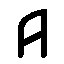
\includegraphics[width=4cm]{images/a2_original.png} }}%
    \qquad
    \subfloat[\centering Зображення із накладеним гаусовим шумом]{{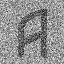
\includegraphics[width=4cm]{images/a2_noised.png} }}%
    \caption{Приклад вхідного зображення, $|T|=4096$}%
    \label{fig:a2_original}
\end{figure}

Для задачі знешумлення використаємо якості вершин 
\begin{equation*}
    q_t(k) = 
    \begin{cases}
        p_t, & k = 0,\\
        255-p_t, & k = 1,
    \end{cases}
\end{equation*}
де $p_t$ --- інтенсивність пікселя в об'єкті $t\in T$, 
і якості ребер
\begin{equation*}
    g_{tt'}(k,k') = K\cdot|k-k'|, \forall tt'\in\Gamma,
\end{equation*}
де $K$---коефіцієнт згладжування.
Якості вершин мінімальні, коли присвоюємо мітку $0$ темним пікселям або мітку $1$ світлим.
Якості ребер відповідають за плавність переходів. Зафіксуємо $K=50$ для прикладів.
На \ref{fig:comparison} порівняємо результати роботи алгоритму із алгоритмом
пошуку максимального потоку (реалізація \cite{Boykov}). Всі обчислення робилися
на комп'ютері з процесором Intel Core i7-10510U і оперативно
запам'ятовуючим пристроєм DDR4 2667MHz. Алгоритм пошуку розв'язує задачу точно \cite{Boykov,Boykov_2,ishikawa,savchynskyy}, тому
значення максимального потоку має співпадати із значенням цільової функції задачі
оптимізації.
\begin{figure}[h]
    \centering
    \subfloat[\centering maxflow (0.004s, $|f|=415612$)]{{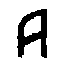
\includegraphics[width=5cm]{images/a2_50.png} }}%
    \qquad
    \subfloat[\centering Запропонований алгоритм (41s, $E(q,g,\varphi)=415612$)]{{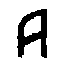
\includegraphics[width=5cm]{images/a2_50.png} }}%

    \subfloat[maxflow (0.004s, $|f|=429022$)]{{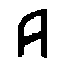
\includegraphics[width=5cm]{images/a2_100.png} }}%
    \qquad
    \subfloat[Запропонований алгоритм (41s, $E(q,g,\varphi)=429022$)]{{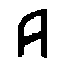
\includegraphics[width=5cm]{images/a2_100.png} }}%
    \caption{Знешумлення, верхній ряд $K=50$, нижній $K=100$}%
    \label{fig:comparison}
\end{figure}